\documentclass[11pt]{article}

\usepackage[a4paper, margin=2.6cm]{geometry}
\usepackage[T1]{fontenc}
\usepackage{lmodern}
\usepackage{microtype}
\usepackage{amsmath}
\usepackage{booktabs}
\usepackage{graphicx}
\usepackage{amssymb}
\usepackage{tikz}
\usetikzlibrary{arrows.meta, positioning, shapes.geometric, fit}
\usepackage{xcolor}
\usepackage[colorlinks=true, linkcolor=black, citecolor=blue!60!black, urlcolor=blue!60!black]{hyperref}
\usepackage{caption}
\captionsetup{font=small, labelfont=bf}

\definecolor{inkblue}{RGB}{40,70,120}
\definecolor{gatered}{RGB}{170,60,55}
\definecolor{leafgreen}{RGB}{60,120,80}

\title{\textbf{Nullius: An Evidence-Gated Architecture for\\ Autonomous Scientific Research on a Local Machine}}
\author{Mikoto Perut\\ Studio Uchu}
\date{July 2026}

\begin{document}

\maketitle

\begin{abstract}
\noindent
Large language models (LLMs)\footnote{A \emph{large language model} is a neural network trained on very large text corpora to predict text. Systems such as GPT and Claude belong to this family. They are fluent but not inherently truthful: they can produce confident statements with no factual basis, a failure mode called \emph{hallucination}.} can now draft research plans, write analysis code, and compose manuscripts, yet evaluations of autonomous ``AI scientist'' systems repeatedly report fabricated or unsupported numbers, unreliable literature handling, and experiments that fail or cannot be reproduced. We present \textsc{Nullius}, a local-first desktop workbench for LLM-driven research whose central design rule is borrowed from the motto of the Royal Society --- \emph{nullius in verba}, ``take nobody's word for it.'' Nullius never trusts model output directly. Every quantitative claim must trace to an artifact produced by locally executed code; every citation must resolve against a bibliographic registry and survive title, author, year, and retraction checks; and every manuscript revision passes through a deterministic gate that rejects untraceable content \emph{before} it is written, even in fully autonomous operation. Generation and verification are separated across independently configured model roles, generated code runs inside a deny-by-default sandbox with resource limits, and a streaming console exposes every prompt, response, and intermediate reasoning trace for audit. We describe the architecture, the integrity gates and the adversarial test suite that guards them, and the concurrency model that parallelizes independent research lanes while keeping a single writer for the shared manuscript. In a controlled case study, the same inexpensive model that silently mis-estimates a regression slope by 35\% when asked directly produces, under Nullius, a sandbox-executed estimate within 0.02\% of truth --- and its one attempt to embellish the manuscript with uncomputed statistics is rejected at the write boundary. We argue that layering cheap, deterministic verification around inherently unreliable generators is a practical recipe for trustworthy machine-assisted science.
\end{abstract}

\begin{center}
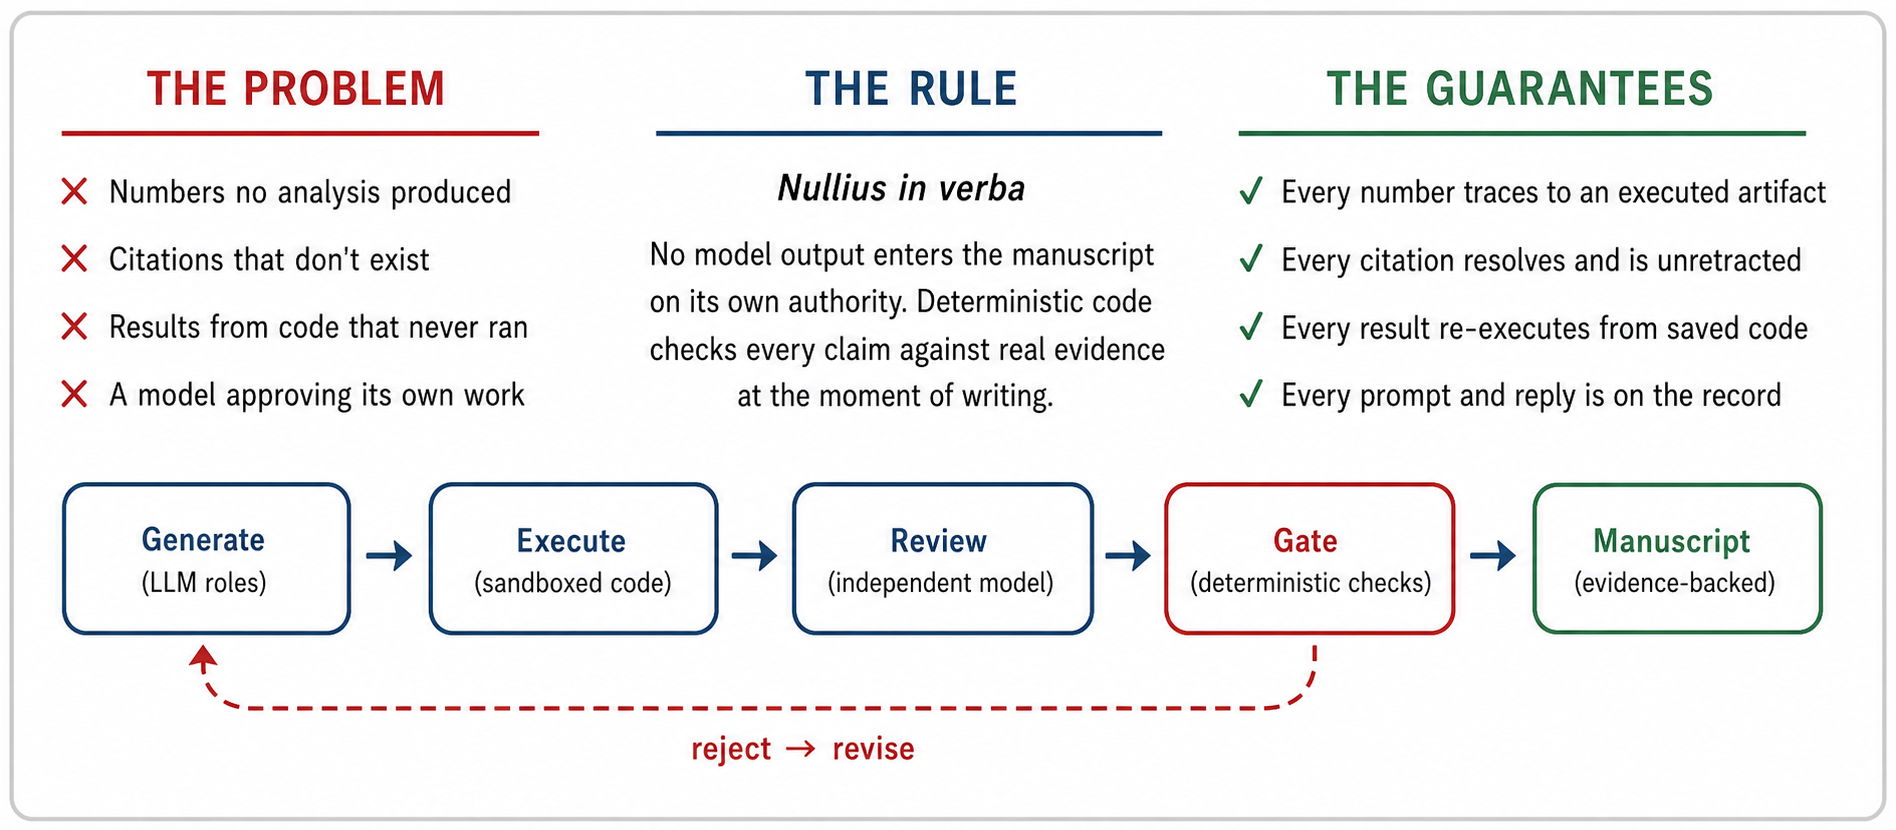
\includegraphics[width=\textwidth]{figures/glance.png}
\captionof{figure}{\textbf{Nullius at a glance.} The recurring failures of autonomous ``AI scientist'' systems (left) are made structurally unavailable by one rule (center): a deterministic gate stands between every model output and the manuscript, backed by sandboxed execution and an independent reviewer (bottom). What survives the gate carries the guarantees on the right.}
\label{fig:glance}
\end{center}

\vspace{1mm}

\section{Introduction}

Recent systems have demonstrated that LLM agents\footnote{An \emph{agent} is an LLM wrapped in a control loop that lets it take actions --- run code, search literature, edit files --- rather than only produce text. A \emph{harness} is the surrounding software that orchestrates those actions.} can carry a research project from question to manuscript with little human input. Independent evaluation, however, documents a discouraging pattern: a substantial share of automatically generated experiments fail outright, literature reviews and novelty assessments are unreliable, and the recurring failures are not exotic. They are fabricated or subtly wrong numbers, citations to papers that do not exist or do not say what is claimed, conclusions drawn from code that was never actually executed, and results that cannot be regenerated from the recorded materials \cite{beel2025}.

These failures share a root cause. An LLM is an excellent \emph{generator} and a poor \emph{witness}: it has no internal distinction between remembering and inventing. Two further results sharpen the problem. First, self-correction without external feedback tends not to help --- a model reviewing its own output shares its own blind spots, and can even revise correct answers into incorrect ones \cite{huang2024}. Second, when LLMs act as evaluators they exhibit systematic biases, including a marked preference for their own generations \cite{judge-bias, self-pref}. A pipeline in which one model writes, the same model reviews, and nothing else checks, is therefore an amplifier of error dressed as a safeguard.

Nullius is built on the opposite premise. The system assumes every model output may be wrong and asks a simple question at each stage: \emph{what non-LLM evidence supports this?} The answer is enforced by construction:

\begin{itemize}
  \item \textbf{Execution is the source of truth.} A ``result'' exists only if locally executed code produced an artifact\footnote{An \emph{artifact} is a concrete file produced by running code --- a CSV table, a JSON summary, a plot image. Artifacts are the ground truth that prose must match.} with exit code~0. Failed runs are never promoted to evidence.
  \item \textbf{Claims are ledgered and gated.} Sentences in the manuscript are registered as typed claims linked to specific evidence, and a deterministic gate --- ordinary code, not a model --- decides what may enter the document.
  \item \textbf{Verification is external and diverse.} Reviewing is performed by an independently configured model role by default, numbers are checked against artifacts by value matching, and citations are checked against the Crossref registry\footnote{\emph{Crossref} is the public registry through which most scholarly publishers assign DOIs (Digital Object Identifiers). Resolving a DOI there proves a work exists and returns its registered title, authors, year, and retraction notices.} rather than against the model's memory.
  \item \textbf{Everything is auditable.} Every prompt, response, and intermediate reasoning trace is streamed live to a console and persisted to disk, together with token and cost accounting.
\end{itemize}

The contribution of this paper is not a new model but a \emph{harness design}: an account of where deterministic checks can be placed around unreliable generators so that the properties users care about --- numbers that are real, citations that resolve, results that reproduce --- are enforced by construction rather than requested by prompt.

\section{Design Principles from the Literature}
\label{sec:principles}

Five findings from recent work directly shaped the architecture.

\paragraph{P1: Do not let the generator grade itself.}
Self-correction studies show that without external signals, LLM revision loops add confidence, not information \cite{huang2024}. Judge studies add that models systematically over-score their own outputs \cite{self-pref}. Nullius therefore separates the \emph{planner}, \emph{executor}, and \emph{reviewer} into independently configured roles --- by default pointing at different providers or model families --- and treats a shared-model configuration as an explicit, discouraged opt-in.

\paragraph{P2: Prefer verification signals a model cannot argue with.}
A reviewer model can be talked out of an objection; a hash cannot. Wherever a property can be checked deterministically --- does this number appear in any artifact, does this DOI resolve, does re-running this code regenerate this file --- Nullius uses plain code and reserves LLM judgment for what genuinely requires it (methodological critique, novelty, prose quality).

\paragraph{P3: Enforce at the write boundary, not after the fact.}
Audits of autonomous research systems observe that the more automated the pipeline becomes, the harder its failures are to see \cite{beel2025}. A check that runs only at final export lets fabricated content live in the manuscript for hours of autonomous operation, contaminating later steps that read it. Nullius runs its gates \emph{when text is written}, so a fabricated value never enters the document at all (Section~\ref{sec:gates}).

\paragraph{P4: Treat generated code as untrusted input.}
Model-written code executes with whatever authority the host grants it, and prompt-injected instructions can arrive through attached files \cite{sandbox-eval}. Nullius runs generated code inside a deny-by-default sandbox with resource limits, and fences file-derived prompt content as data rather than instructions (Section~\ref{sec:substrate}).

\paragraph{P5: Make the machine's work observable.}
Trust in autonomous systems tracks what the operator can inspect \cite{anthropic-agents}. Nullius streams every model interaction --- including intermediate reasoning tokens where providers expose them --- to a live console, and archives complete transcripts keyed by run.

\section{Architecture}
\label{sec:arch}

\begin{figure}[t]
\centering
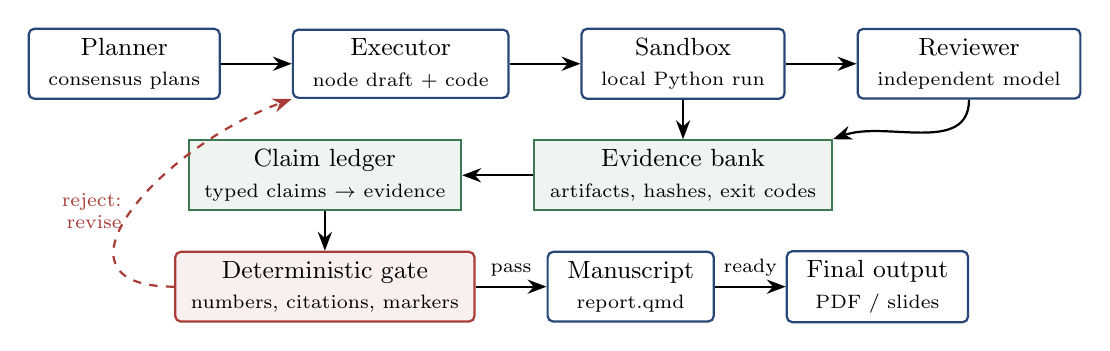
\begin{tikzpicture}[
  font=\small,
  node distance=5mm and 9mm,
  box/.style={draw=inkblue, thick, rounded corners=2pt, align=center, minimum height=8.5mm, inner xsep=2.5mm},
  gate/.style={draw=gatered, thick, rounded corners=2pt, align=center, fill=gatered!8, minimum height=8.5mm, inner xsep=2mm},
  store/.style={draw=leafgreen, thick, align=center, fill=leafgreen!8, minimum height=8.5mm, inner xsep=2mm},
  arr/.style={-{Stealth[length=2.4mm]}, thick}
]
\node[box] (plan) {Planner\\\scriptsize consensus plans};
\node[box, right=of plan] (exec) {Executor\\\scriptsize node draft + code};
\node[box, right=of exec] (sand) {Sandbox\\\scriptsize local Python run};
\node[box, right=of sand] (rev) {Reviewer\\\scriptsize independent model};
\node[store, below=of sand] (bank) {Evidence bank\\\scriptsize artifacts, hashes, exit codes};
\node[store, left=of bank] (ledger) {Claim ledger\\\scriptsize typed claims $\to$ evidence};
\node[gate, below=of ledger] (gate) {Deterministic gate\\\scriptsize numbers, citations, markers};
\node[box, right=of gate] (qmd) {Manuscript\\\scriptsize report.qmd};
\node[box, right=of qmd] (out) {Final output\\\scriptsize PDF / slides};

\draw[arr] (plan) -- (exec);
\draw[arr] (exec) -- (sand);
\draw[arr] (sand) -- (rev);
\draw[arr] (sand) -- (bank);
\draw[arr] (rev.south) to[out=-90,in=20] (bank.north east);
\draw[arr] (bank) -- (ledger);
\draw[arr] (ledger) -- (gate);
\draw[arr] (gate) -- node[above, font=\scriptsize]{pass} (qmd);
\draw[arr] (qmd) -- node[above, font=\scriptsize]{ready} (out);
\draw[arr, dashed, gatered] (gate.west) to[out=180,in=200,looseness=1.6] node[left, font=\scriptsize, align=right]{reject:\\revise} (exec.south west);
\end{tikzpicture}
\caption{The Nullius pipeline. Model roles (blue) generate; the sandbox executes; artifacts and their hashes accumulate in the evidence bank (green); and a deterministic gate (red) --- plain code, not a model --- decides what may be written into the shared manuscript. Rejected content loops back for revision instead of entering the document.}
\label{fig:pipeline}
\end{figure}

\subsection{Roles, lanes, and nodes}

A Nullius project begins with a research question, optional theory and protocol files, and data. A \emph{planner} role proposes candidate plans; executor and reviewer roles critique them; and the planner synthesizes a consensus plan --- a lightweight debate that produces plans with explicit observables, success criteria, and \emph{falsification criteria}\footnote{A falsification criterion states in advance what result would count \emph{against} the hypothesis. Fixing it before running any analysis is a classic guard against ``HARKing'' --- hypothesizing after the results are known.}. Adopted plans are frozen into a \emph{protocol lock}; changing the plan afterwards records an amendment that blocks final output until a human approves it.

Each adopted plan spawns a \emph{lane}: an autonomous researcher with its own folder on disk. Lanes grow as chains of \emph{nodes}, where one node is one concrete step --- a question, generated Python code, an execution record, artifacts, and an independent review. Nodes carry explicit prerequisite links, so the workspace is a dependency graph\footnote{Formally a \emph{directed acyclic graph} (DAG): steps point at the steps they depend on, and no step can depend on itself through a cycle.} whose structure the scheduler exploits (Section~\ref{sec:concurrency}).

\subsection{The evidence bank and the claim ledger}

Executing a node's code inside the sandbox produces artifacts. Each successful run is recorded in the \emph{evidence bank} with the producing command, exit code, artifact paths, and SHA-256 hashes\footnote{A \emph{hash} is a short fingerprint computed from a file's bytes. If the file changes in any way, the fingerprint changes, so hashes make silent modification detectable.}. Failed runs are explicitly \emph{not} promoted: an artifact left behind by a crashed script cannot support a claim.

When the synthesizer role drafts manuscript text, it must declare its factual sentences as typed \emph{claims} --- result, background, methodological, limitation, or interpretation --- each pointing at supporting evidence. The claim ledger is the bridge between prose and ground truth: a result claim is admissible only when its primary support is execution evidence with exit code~0; a background claim only when its citation is verified (Section~\ref{sec:gates}). Claims whose named evidence cannot be resolved are marked unsupported and cannot enter the document.

\section{Deterministic Integrity Gates}
\label{sec:gates}

The gates are ordinary functions over project state --- no model in the loop --- and they run at two points: at the \emph{write boundary}, whenever a manuscript patch is staged, and at \emph{readiness}, before final output. Table~\ref{tab:gates} summarizes them.

\begin{table}[t]
\centering
\small
\begin{tabular}{@{}p{0.23\textwidth}p{0.51\textwidth}p{0.17\textwidth}@{}}
\toprule
\textbf{Gate} & \textbf{What it checks} & \textbf{On failure} \\
\midrule
Numeric grounding & Every decimal in Results/Abstract/Discussion matches, at its own precision, a value parsed from a real artifact; standalone integers are tracked in a softer advisory bucket & blocks the patch \\
Citation verification & Every cited work's DOI resolves in Crossref; registered title (symmetric token match), authors, and year agree; retraction notices are detected & blocks the patch \\
Execution provenance & Result claims trace to a run with exit code~0; hand-attached ``results'' without an execution record are rejected & claim inadmissible \\
Marker \& leak scan & No unresolved \texttt{[citation needed]}/\texttt{[execution needed]} markers; no internal tooling vocabulary leaks into prose & blocks the patch \\
Reproducibility & Re-running each node's saved code in a clean staging copy (recorded artifacts removed first) regenerates equivalent artifacts under a numeric-canonical comparison & blocks readiness \\
Protocol integrity & Post-lock plan changes require explicit human approval & blocks readiness \\
\bottomrule
\end{tabular}
\caption{The deterministic gates. ``Blocks the patch'' means the offending text never enters the manuscript, even under fully autonomous operation; ``blocks readiness'' means final output cannot be produced until the issue is resolved.}
\label{tab:gates}
\end{table}

\subsection{Numeric grounding without loopholes}

The naive check --- ``does the number appear as a substring of any artifact?'' --- is exploitable: a fabricated $0.87$ would be ``grounded'' by an unrelated $10.873$ in a CSV. Nullius instead parses artifacts into numeric \emph{values} and asks whether any value rounds to the reported number at the number's own printed precision, with percent forms matched against their $/100$ equivalents. Substring matching is deliberately absent. The check covers the Results section and also the Abstract and Discussion, where headline numbers are routinely restated. Integers are handled in a separate advisory bucket (fabricated sample sizes matter, but phrases like ``95\% CI'' make hard-blocking on integers too noisy); they weigh on the readiness score at half strength.

\subsection{Citation verification beyond existence}

The characteristic LLM citation failure is not an obviously fake reference but a \emph{plausible} one \cite{beel2025}. The gate therefore requires more than resolution: the locally recorded title must match the registered title under a symmetric Dice coefficient\footnote{The Dice coefficient between two token sets $A,B$ is $2|A\cap B|/(|A|+|B|)$. Being symmetric, it rejects the spoof where a short generic title (``Deep Learning'') hides inside a long real one.} with a length-ratio guard, at least one author family name must overlap, a year discrepancy beyond one is rejected, and Crossref retraction relations mark the work as \emph{retracted} and permanently inadmissible. User-imported references are honored only if they carry a resolvable pointer (DOI or URL) --- a bare title is indistinguishable from a fabrication. An optional advisory layer fetches the cited work's abstract and asks the reviewer role whether it supports the specific claim; because this judgment is itself an LLM output, it annotates but never gates.

\subsection{Reproducibility as re-execution}

Before final output, Nullius re-runs every node's saved code in an isolated staging copy from which the recorded artifacts have been \emph{removed} --- so a script that merely fails to overwrite stale outputs is caught as ``not regenerated'' rather than passing by accident. Regenerated artifacts are compared bytewise, with a numeric-canonical fallback for text artifacts (parsed values at ten significant digits plus a number-masked skeleton) so that timestamp or float-formatting differences do not raise false alarms.

\subsection{Adversarial regression tests}

Every gate ships with red-team tests encoding its known bypasses: the substring collision, the subset-title spoof, the sourceless user import, the stale-artifact reproduction, the fabricated patch under autonomous auto-apply, and mocked registry responses for match, mismatch, missing, and retracted cases. The suite exists because each of these was a real hole in an earlier revision; the tests keep them closed.

\section{Execution Substrate and Observability}
\label{sec:substrate}

\paragraph{Sandboxed execution.}
Generated Python runs under a deny-by-default macOS sandbox profile: reads of the user's home directory are blocked except the node folder and the Python runtime itself, writes are confined to the node folder and temporary directories, the network is blocked by default, and POSIX resource limits\footnote{Set via \texttt{ulimit}: caps on CPU seconds, virtual memory, and file size, so a runaway loop or memory bomb dies from its limits instead of taking the machine down.} apply inside the sandbox. If the sandbox facility is unavailable, execution is \emph{refused} rather than silently downgraded; running unsandboxed requires a deliberate setting change. Prompt content extracted from attached files is wrapped in explicit untrusted-data fences with a standing rule that fenced content is data to analyze, never instructions to follow --- closing the classic injection path from a poisoned PDF to locally executed code.

\paragraph{Reliable transport.}
All API traffic passes through one policy layer: transient failures (HTTP 429/5xx, flaky networks) retry with exponential backoff honoring \texttt{Retry-After}; authentication and malformed-request errors fail fast with typed messages; and truncated generations are detected from the provider's finish reason instead of surfacing as mysterious parse errors. Token usage is captured per call and converted to cost using live model pricing.

\paragraph{The mission console.}
A dedicated dark console streams every model interaction in real time --- output tokens with a live caret, and, where providers expose them, intermediate \emph{reasoning} tokens in a separate collapsible track --- with per-call token, cost, and latency badges. Full prompts, responses, and reasoning traces are archived as append-only JSONL\footnote{\emph{JSON Lines}: a log format with one JSON record per line, easy to append to and to replay.} transcripts keyed by run ID; the console lazy-loads them on demand so the interface stays responsive over long sessions. Streaming updates are coalesced to $\sim$15\,Hz so rendering cost stays constant regardless of token rate. The console is not cosmetic: it is the operator's instrument for catching drift early and the audit trail for reconstructing exactly what the machine was told and what it answered.

\paragraph{Human-in-the-loop steering.}
Observability exists so that intervention is possible, and intervention is a first-class mechanism rather than an emergency stop. An autonomous run \emph{pauses itself} at defined checkpoints --- a failed execution that automatic repair could not fix, or an accumulation of unresolved critical reviews --- and presents the operator with concrete recovery actions: resume, rerun the offending node, trigger a supervised self-correction, or continue while explicitly leaving the failed node marked as unverified evidence. The operator can also stop a run at any moment (running child processes are terminated immediately), inject steering instructions that subsequent planning steps must read, and approve or reject every staged manuscript patch and every post-lock protocol amendment. The division of labor is deliberate: the gates automate what can be decided mechanically, and everything that requires judgment is routed to the human at the moment it arises, with the full transcript at hand to inform the decision.

\section{Concurrency: Parallel Where Independent, Serial Where Shared}
\label{sec:concurrency}

Autonomous research is dominated by waiting --- on model responses and on local runs. Nullius exploits the lane structure: a scheduler selects lanes whose prerequisites are settled, and their next nodes are \emph{produced} (generated and executed) concurrently, since lanes live in disjoint folders and share no intermediate state. \emph{Application} of the produced nodes --- review, self-correction, and the update of the shared manuscript --- remains strictly serial in lane order, because the manuscript is a single document whose patches are validated against a base-content hash; a single writer keeps that validation meaningful. This produce-parallel/apply-serial split captures most of the available speedup ($N$ lanes wait together instead of one after another) without weakening any gate. Persistence is incremental --- only the changed lane's workspace is rewritten per step --- and a user stop terminates running child processes immediately through a process registry rather than waiting out a long run.

Self-correction, when the reviewer requests it, is bounded and grounded: revision rounds are capped, execution results take precedence over rhetorical responses, and the loop exits to a human when the model reports it needs input --- reflecting the evidence that unbounded self-revision does not converge \cite{huang2024}.


\section{From Prototype to Product: A Cross-Platform Implementation}
\label{sec:implementation}

The architecture above was first realized as a native macOS application. To make the harness usable beyond one operating system, we reimplemented it as a TypeScript monorepo: a headless core engine, a command-line interface, a local server that exposes the engine over HTTP and WebSocket, and a desktop application (Tauri~+~React) that connects to that server. Nothing in the gate semantics changed --- and this is not an assertion but a tested property: the original test suite was ported into \emph{language-independent conformance vectors} (JSON files pairing inputs with required verdicts, including the adversarial cases of Section~6.4), and the new engine must reproduce every verdict bit-for-bit. The vectors, not either implementation, are the specification.

The execution substrate gained a notable property in translation. The default sandbox is now \emph{WebAssembly}\footnote{WebAssembly (WASM) is a portable binary format executed inside a memory-isolated virtual machine. Code compiled to WASM can only touch the outside world through functions the host explicitly provides.}: generated Python runs on a CPython interpreter compiled to WASM (Pyodide), inside a worker thread with a hard timeout. Isolation is not a policy applied to the process but a property of the substrate --- the sandbox exposes no network functions, so exfiltration is not forbidden merely; it is inexpressible. This also removes the last installation barrier: the default path needs no container runtime and works identically on Windows, Linux, and macOS, with the native deny-by-default sandbox and an optional container backend available where full CPython compatibility is required. The refusal principle is preserved: if no sandbox can be established, execution is refused, never silently downgraded.

Three workflow details matter in practice. First, \emph{user data}: files placed in the project's \texttt{data/} folder (or added through the desktop application) are copied read-only into every run's working directory, and the executor role is instructed to base its analysis on them --- absent such files, it must generate the data its plan requires. Second, \emph{automation}: the command-line interface exposes the full loop (\texttt{init}, \texttt{plan}, \texttt{adopt}, \texttt{run}, \texttt{steer}, \texttt{approve}/\texttt{reject}, \texttt{export}), and \texttt{nullius verify --json} emits the complete gate report with a conventional exit code, so a research repository can enforce ``no ungrounded number enters \texttt{main}'' the same way software repositories enforce passing tests. Third, \emph{agent supervision}: external coding agents such as Codex, Claude Code, and OpenCode can drive the same CLI without being embedded in the desktop application. Each CLI command appends a structured event to the project's activity journal; the local server tails that journal and streams the events into the desktop live-activity pane. Thus the operator can watch an external agent's verifiable actions --- commands, exit codes, gate results, sandbox failures, readiness changes --- in the GUI even while the agent itself runs in a separate terminal or TUI. The desktop application layers a supervision surface over the same server: a setup path ordered as keys $\rightarrow$ project $\rightarrow$ plan adoption, a live activity pane that streams every model's output and reasoning tokens as they are produced, staged patches rendered with their gate warnings and approve/reject controls, and a readiness board showing each gate as a light. API keys live in the operating-system keychain or process memory only; they are never written to project files.

\section{Case Study: Gated versus Ungated Generation}
\label{sec:casestudy}

Section~\ref{sec:concurrency} argued architecturally; here we observe the difference directly. The protocol is deliberately small and fully reproducible from the repository (\texttt{docs/paper/evaluation/}). We generated a 40-point dataset $y = 3.0x + 1.5 + \varepsilon$, $\varepsilon \sim \mathcal{N}(0, 0.35)$, and asked one inexpensive model (\texttt{gpt-4o-mini}) the same question through two routes: \emph{raw}, a single API call given the CSV inline and asked for a short results report; and \emph{gated}, the same model driving all three Nullius roles with the CSV in the project's \texttt{data/} folder.

The raw route answered fluently and wrongly. Performing regression ``in its head,'' the model reported a slope of $1.9450$ against a true value of $3.0$ --- a 35\% error --- decorated with an intercept, a coefficient of determination\footnote{$R^2$ measures the fraction of variance in $y$ explained by the fitted model; $R^2=1$ is a perfect fit. Reporting a high $R^2$ for a badly wrong slope is exactly the kind of fluent-but-false output that cannot be caught by reading the text alone.} of $0.9985$, and correct-sounding prose. Auditing that report with the numeric-grounding gate (against an empty evidence bank, since nothing was executed) flags every quantitative claim as untraceable.

The gated route surfaced two \emph{different} failures --- and absorbed both. The executor's first program crashed; one bounded self-correction round, prompted by the reviewer's findings and the interpreter's error text, produced a working ordinary-least-squares implementation whose artifact recorded a slope of $3.0007$ (0.02\% from truth). The synthesizer then drafted a manuscript that embedded the artifact's numbers correctly \emph{and added} a significance threshold and an effect figure ($0.05$, $0.7$) that no code had computed. The write-boundary gate rejected the patch --- the manuscript remained empty --- and the console showed why. One steering instruction (``report only numbers present in the artifact; compute $R^2$ explicitly if you wish to report it'') and one rerun later, the manuscript contained slope $3.0007$, intercept $1.4877$, and $R^2 = 0.9997$, every figure traceable; the human rejected the blocked draft, and \texttt{verify} exited 0 with a readiness score of 1.0.

\begin{table}[h]
\centering
\small
\begin{tabular}{@{}lll@{}}
\toprule
 & \textbf{Raw API call} & \textbf{Nullius (same model)} \\
\midrule
Slope estimate (truth: 3.0) & 1.9450 \; (35\% error) & 3.0007 \; (0.02\% error) \\
How computed & in-context ``mental'' arithmetic & sandboxed OLS execution \\
$R^2$ reported & 0.9985 (never computed) & 0.9997 (computed, in artifact) \\
Numbers traceable to evidence & 0 of 5 & all \\
Fabricated additions & undetectable by design & blocked at the write boundary \\
Machine-checkable verdict & none & \texttt{verify} exit 0, score 1.0 \\
\bottomrule
\end{tabular}
\caption{One model, one dataset, one question, two routes. The raw route fails silently; the gated route fails \emph{visibly} twice (a crash, then an embellished draft), recovers under its own machinery, and terminates in a state a script can certify.}
\label{tab:casestudy}
\end{table}

\paragraph{A second comparison: coding-agent harnesses.}
The preceding experiment compares a raw API call with the same API accessed through Nullius. A complementary comparison is more relevant to practitioners who already use coding-agent harnesses: \emph{Codex alone} versus \emph{Codex driving the Nullius CLI}. We therefore ran a second small measurement using a 40-row CSV with the same ordinary-least-squares target. The Codex-alone condition used \texttt{codex-cli 0.141.0} with the local default model configuration, \texttt{gpt-5.5} and \texttt{model\_reasoning\_effort=xhigh}. Codex was asked to analyze the CSV and write \texttt{report.md} directly, without Nullius. It executed code and reported the correct fitted values: slope $2.9988$, intercept $1.5142$, and $R^2=0.9999$. However, when that finished report was imported into a blank Nullius project for audit, \texttt{nullius verify --json} returned \texttt{ok: false}, readiness $0.4214$, zero supported claims, 18 ungrounded floating-point quantities, and three ungrounded integers. The report was accurate in this instance, but the accuracy was not a machine-checkable property of the saved research state.

In the second condition, a Codex coding agent used the Nullius CLI locally: \texttt{init} created a project, a saved analysis script regenerated \texttt{artifacts/regression-results.csv}, execution evidence and result claims were recorded in the project ledger, and \texttt{verify --json} was run on the resulting project. The fitted values were the same to the displayed precision: sample size 40, slope $2.998794063977$, intercept $1.514186251220$, and $R^2=0.999922484256$. This time \texttt{verify} returned \texttt{ok: true}, readiness $1.0$, two supported result claims, no ungrounded result numbers, no stale support references, and no missing artifacts. The evaluation artifacts are archived under \texttt{docs/paper/evaluation/}. To avoid disclosing the repository to a second external Codex subprocess, the CLI condition used the current Codex agent driving the public CLI and project files locally; it did not require embedding Codex's TUI in Nullius.

\begin{figure}[h]
\centering
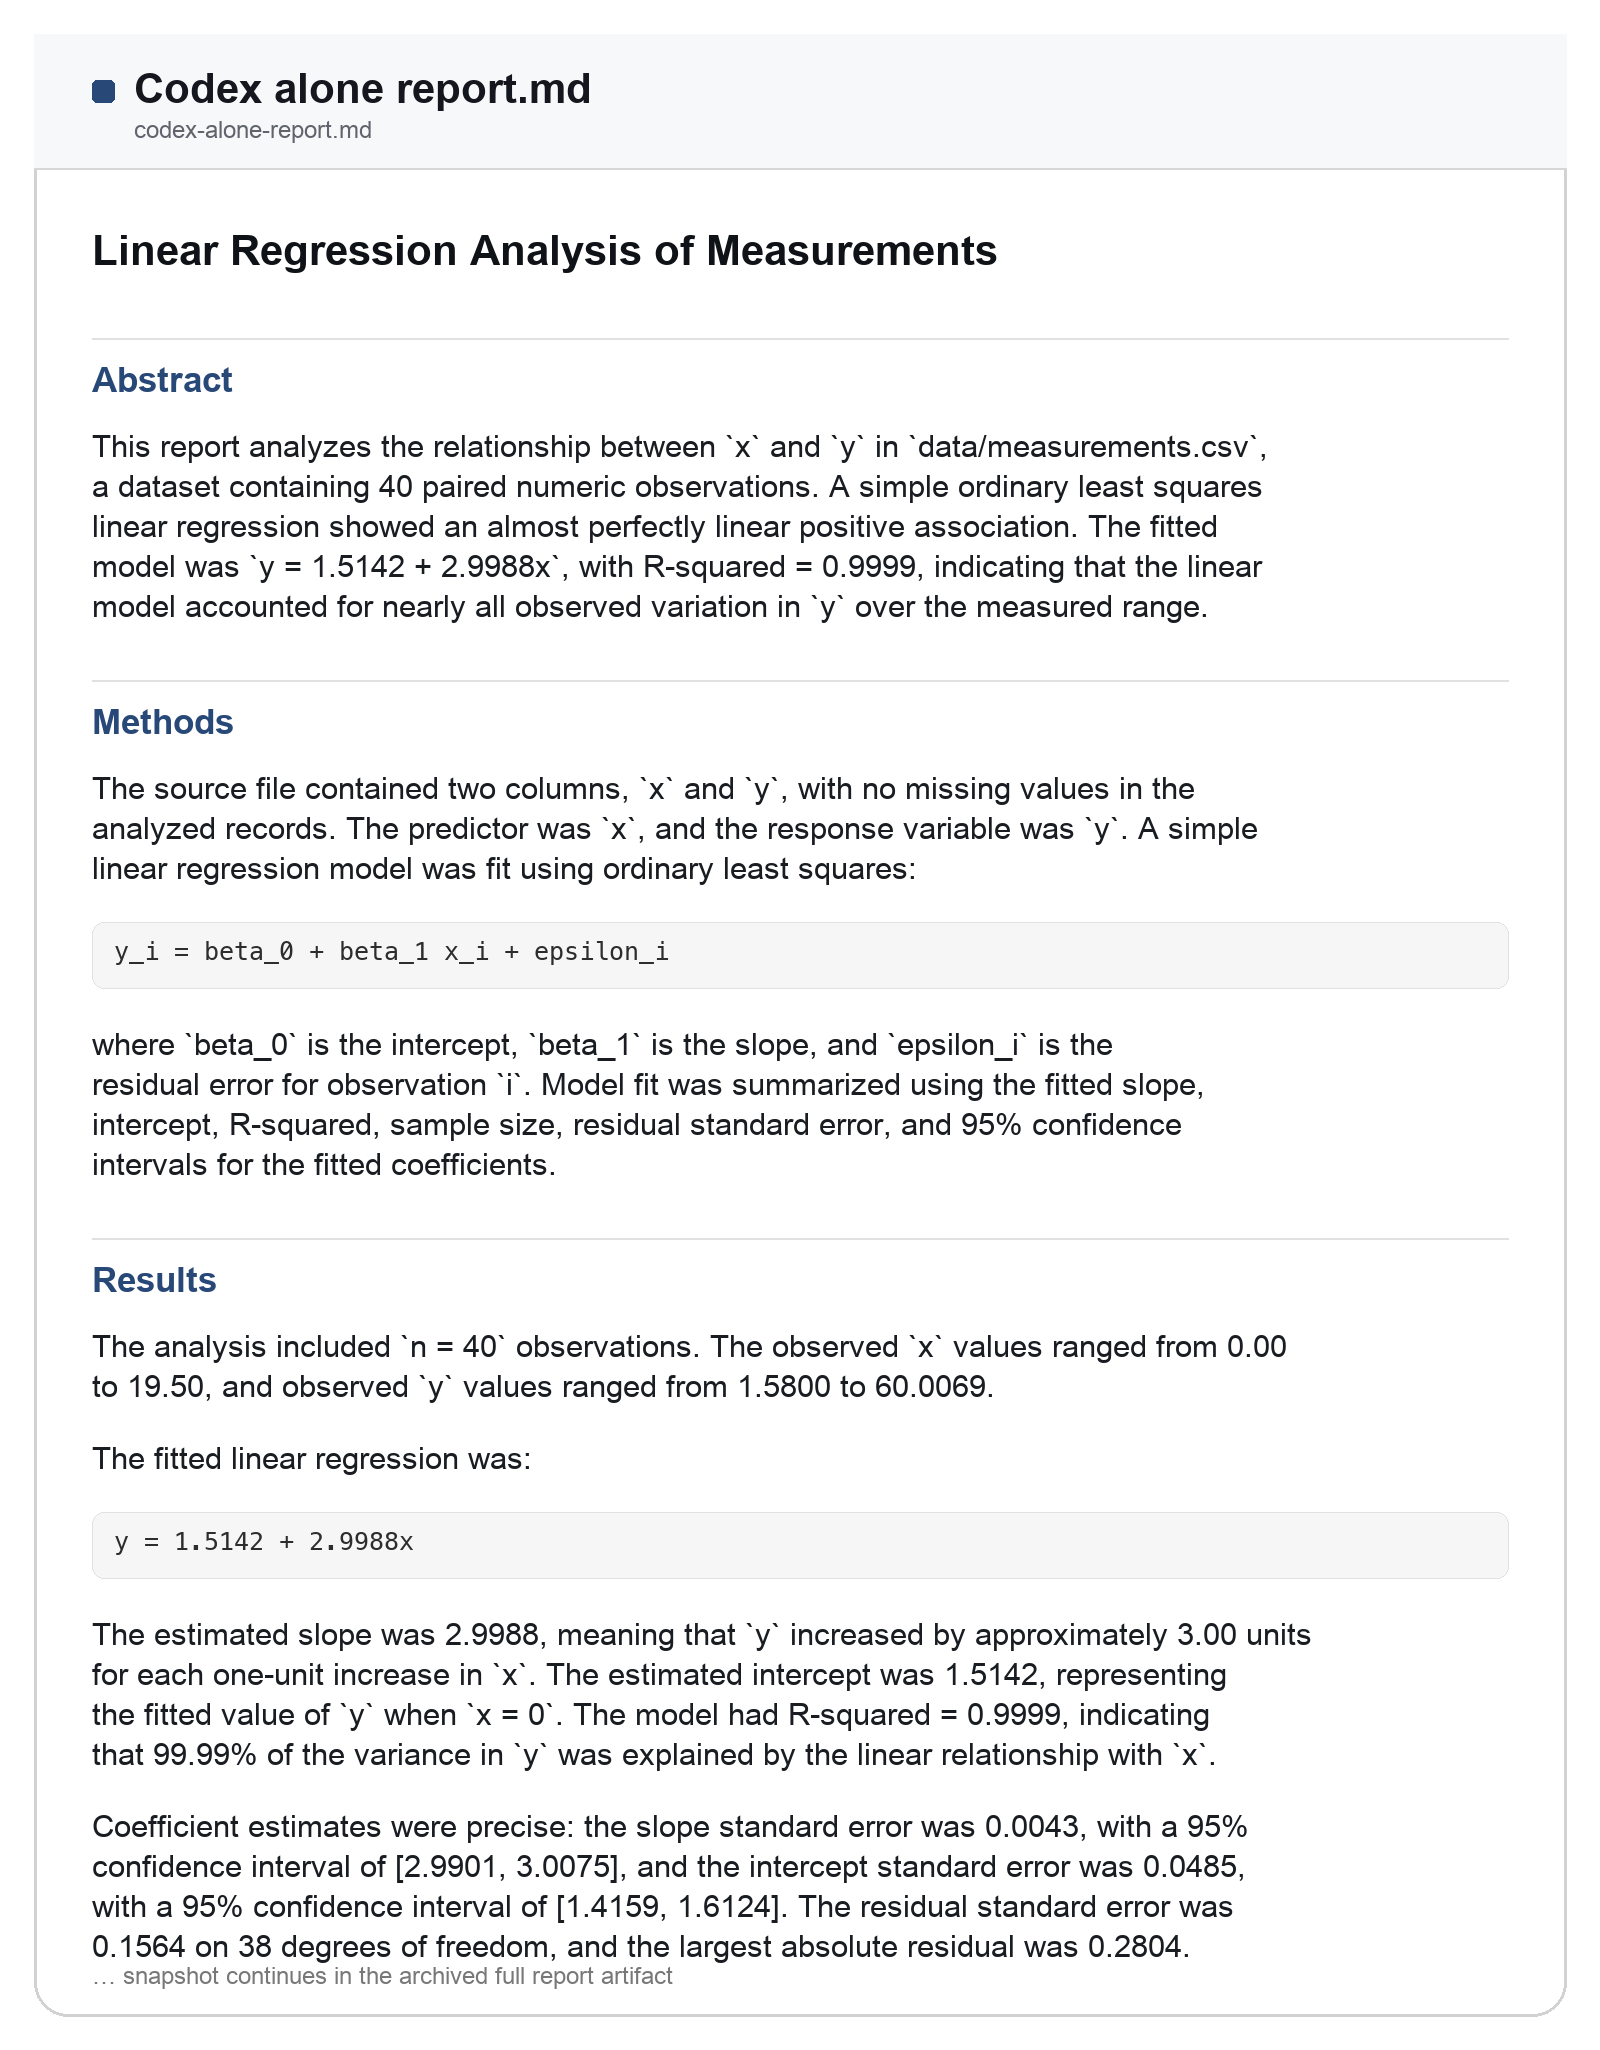
\includegraphics[width=0.48\textwidth]{figures/codex-simple-alone-report-snapshot.png}\hfill
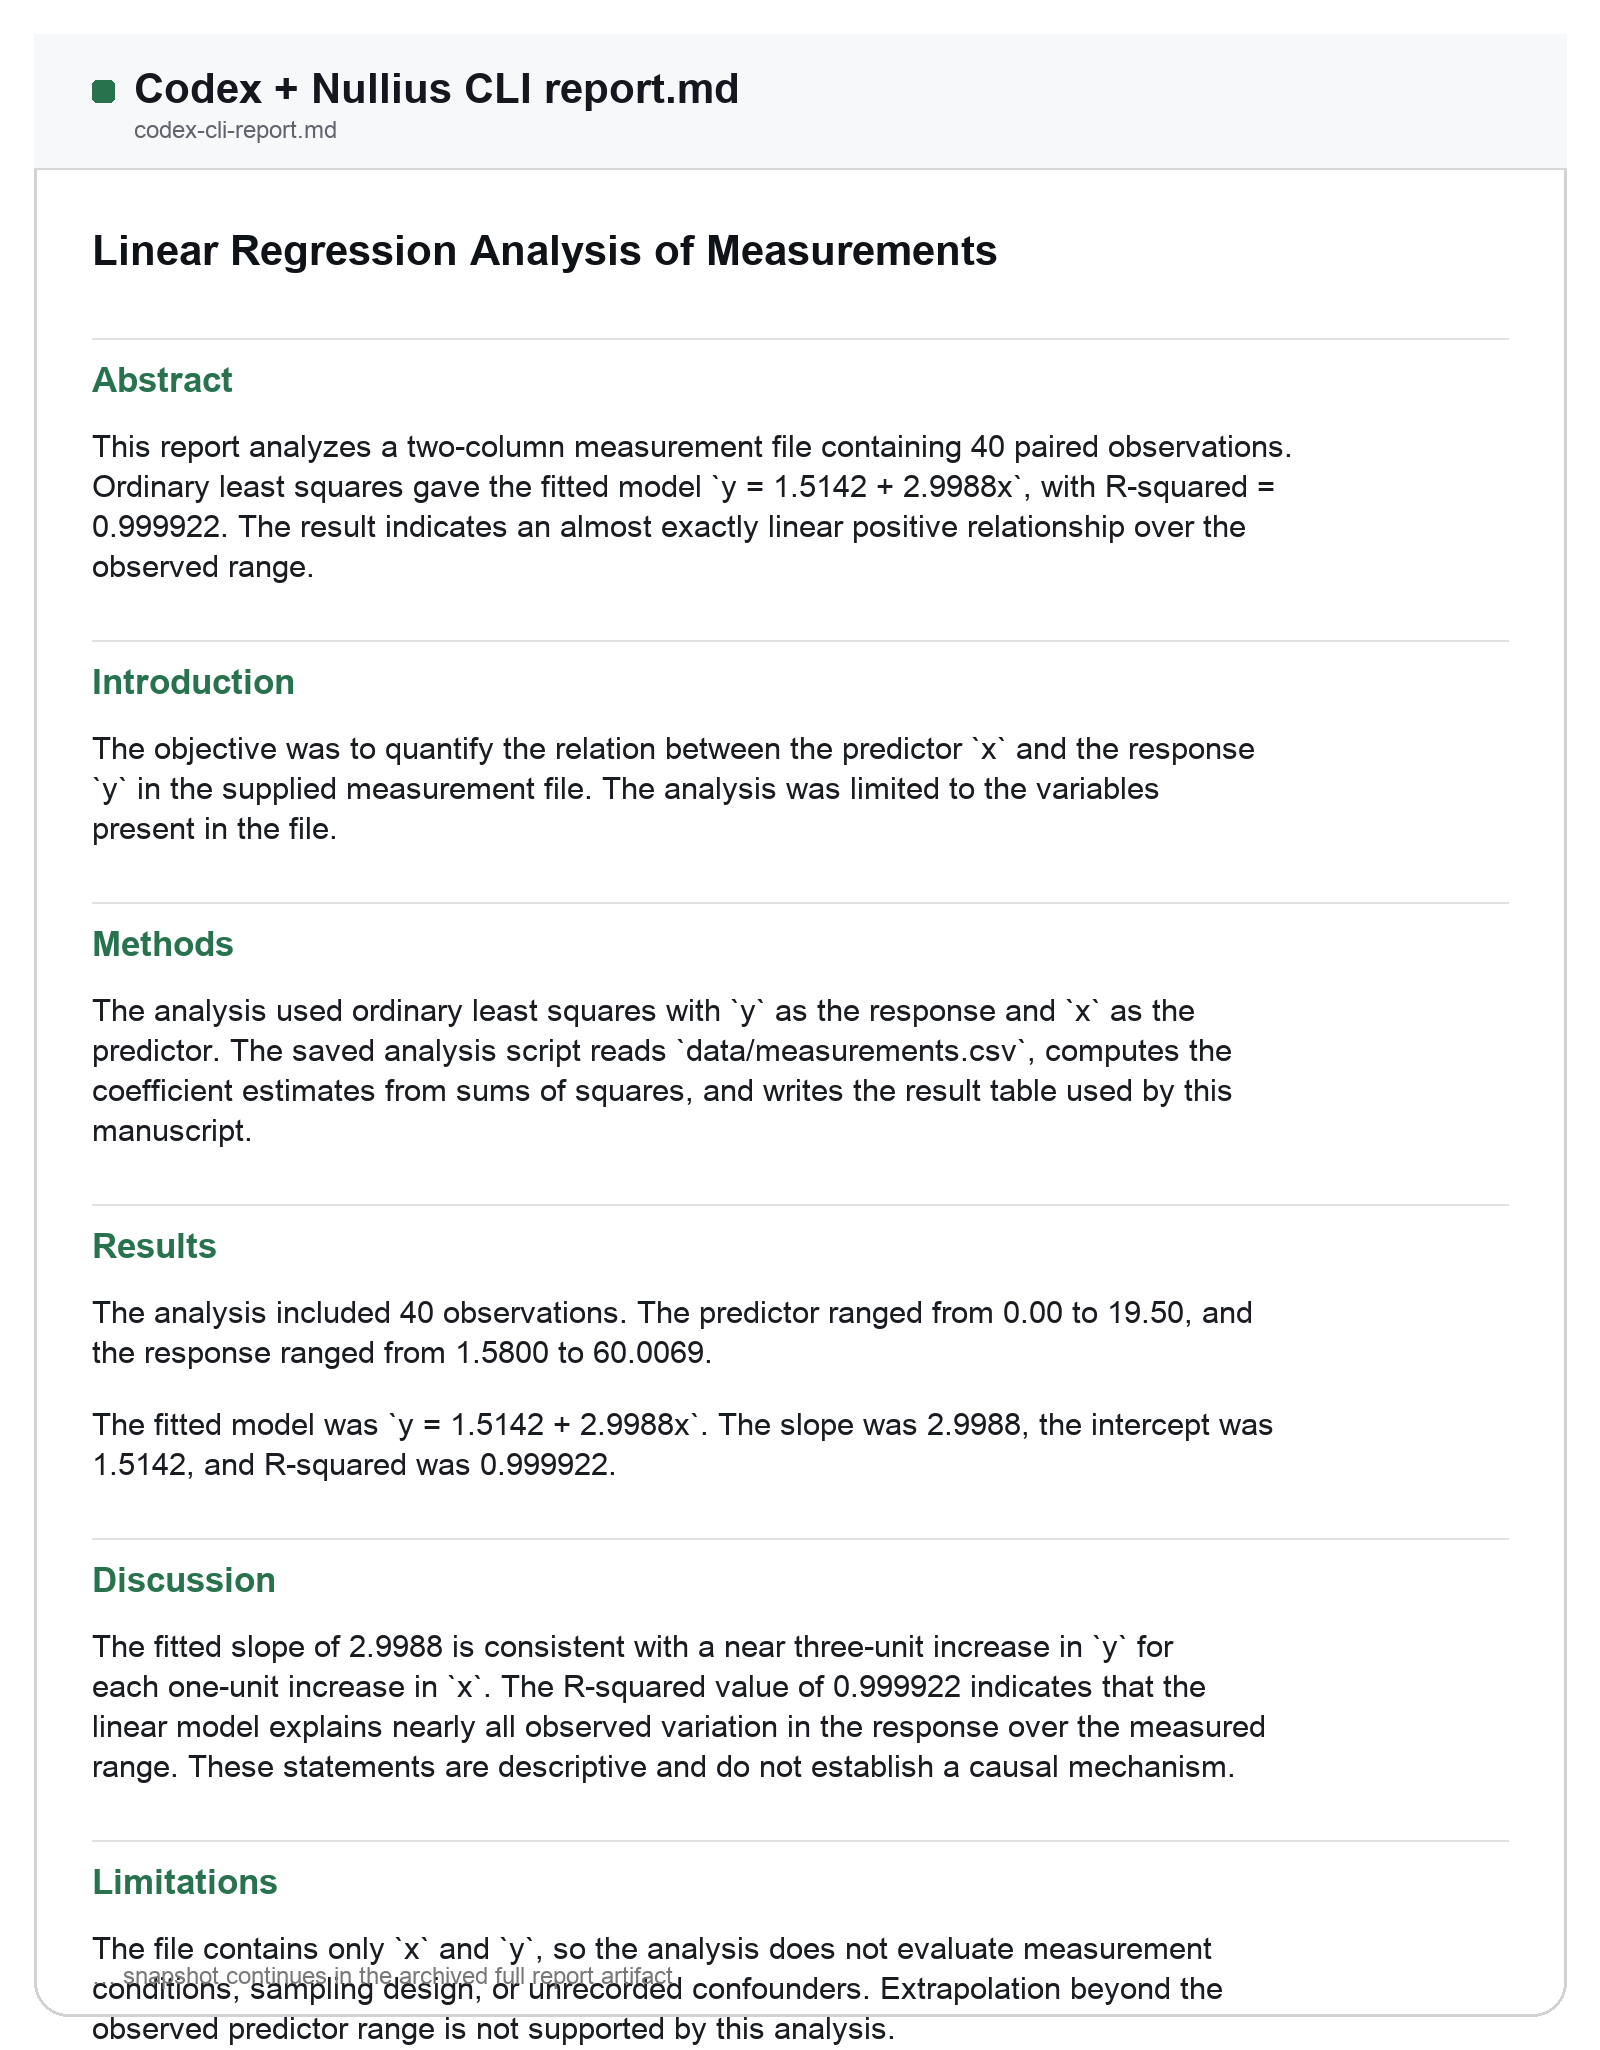
\includegraphics[width=0.48\textwidth]{figures/codex-simple-nullius-report-snapshot.png}
\caption{Rendered snapshots of the two generated reports for the simple harness comparison. Left: the direct Codex report. Right: the report generated from the Nullius project state. Both reports describe the same fitted line to the displayed precision, but they are different research objects: the left report is a standalone narrative, whereas the right report is a projection from executable evidence and a claim ledger.}
\label{fig:codex-simple-report-snapshots}
\end{figure}

The two simple reports differ mostly in their \emph{persistence contract}, not in their scientific conclusion. The Codex-alone report is more expansive as prose: it includes confidence intervals, residual standard error, the largest absolute residual, and a broader limitations paragraph. The Nullius-backed report is more compact and more procedural: it names the saved analysis script and the result artifact used for numeric checking. Both reports state the same fitted relationship to the displayed precision, but only the Nullius-backed report is connected to ledger entries that make the manuscript auditable by \texttt{verify}.

\begin{table}[h]
\centering
\small
\begin{tabular}{@{}p{0.25\textwidth}p{0.33\textwidth}p{0.33\textwidth}@{}}
\toprule
 & \textbf{Codex alone} & \textbf{Codex + Nullius CLI} \\
\midrule
Computed result & $n=40$, slope $2.9988$, intercept $1.5142$, $R^2=0.9999$ & $n=40$, slope $2.998794063977$, intercept $1.514186251220$, $R^2=0.999922484256$ \\
Saved research state & \texttt{report.md} plus the input CSV; no evidence ledger or claim ledger & project manifest, analysis script, result artifact, source activity, execution evidence, two approved result claims \\
After-the-fact audit & \texttt{verify} failed: readiness $0.4214$, supported claims 0 & \texttt{verify} passed: readiness $1.0$, supported claims 2 \\
Numeric grounding & 18 floating-point values and 3 integers ungrounded & 0 ungrounded result numbers, 0 ungrounded integers \\
Failure signal & Correctness had to be judged by inspecting Codex's transcript and recomputing externally & Correctness was represented as a CLI exit code and a machine-readable readiness report \\
Interpretation & Codex can solve the task, but the saved report alone is not a verifiable research object & The same agent work becomes a durable, gate-checkable research object \\
\bottomrule
\end{tabular}
\caption{Measured harness-level comparison on the same synthetic regression file. Codex was competent in both conditions; the difference is not model intelligence but whether the finished state contains executable evidence, supported claims, and a deterministic readiness verdict.}
\label{tab:codexcli}
\end{table}

\paragraph{Comparison 2: a harder multi-table analysis.}
To stress the distinction between coding competence and research-state verification, we repeated the harness comparison on a more demanding synthetic task. The input consisted of three CSV files with 240 joined patients, 18 missing 12-week outcomes, baseline covariates, site indicators, treatment, and a high-CRP biomarker flag. The requested analysis required a complete-case join, an adjusted ordinary-least-squares model for \texttt{outcome\_12w} using treatment, baseline score, age, sex, site, and baseline CRP, and a second model with a treatment-by-high-CRP interaction. The Codex-alone run was invoked explicitly as \texttt{codex exec -m gpt-5.5 -c model\_reasoning\_effort=xhigh}. It detected that \texttt{statsmodels} was unavailable, implemented OLS with \texttt{numpy}/\texttt{scipy}, found and corrected an interpretation error in its own draft, then made the saved script pass \texttt{python3 -W error}.

Both conditions therefore reached the same substantive analysis result. The equality is best stated as \emph{same estimates to the reported precision}, not byte-identical prose. The complete-case count ($n=222$), treatment estimate ($-5.053$), standard error ($0.209$), confidence interval ($[-5.465,-4.641]$), $R^2$ ($0.885$), RMSE ($1.505$), and interaction estimate ($-1.235$) matched to the displayed precision. The textual reporting differed only in precision choices: for example, the Codex-alone report wrote the primary $p$-value as $p<0.001$ and the interaction $p$-value as $p=0.006$, whereas the Nullius manuscript reported the same calculations as $p=3.89\times10^{-63}$ and $p=0.006429$.

\begin{figure}[h]
\centering
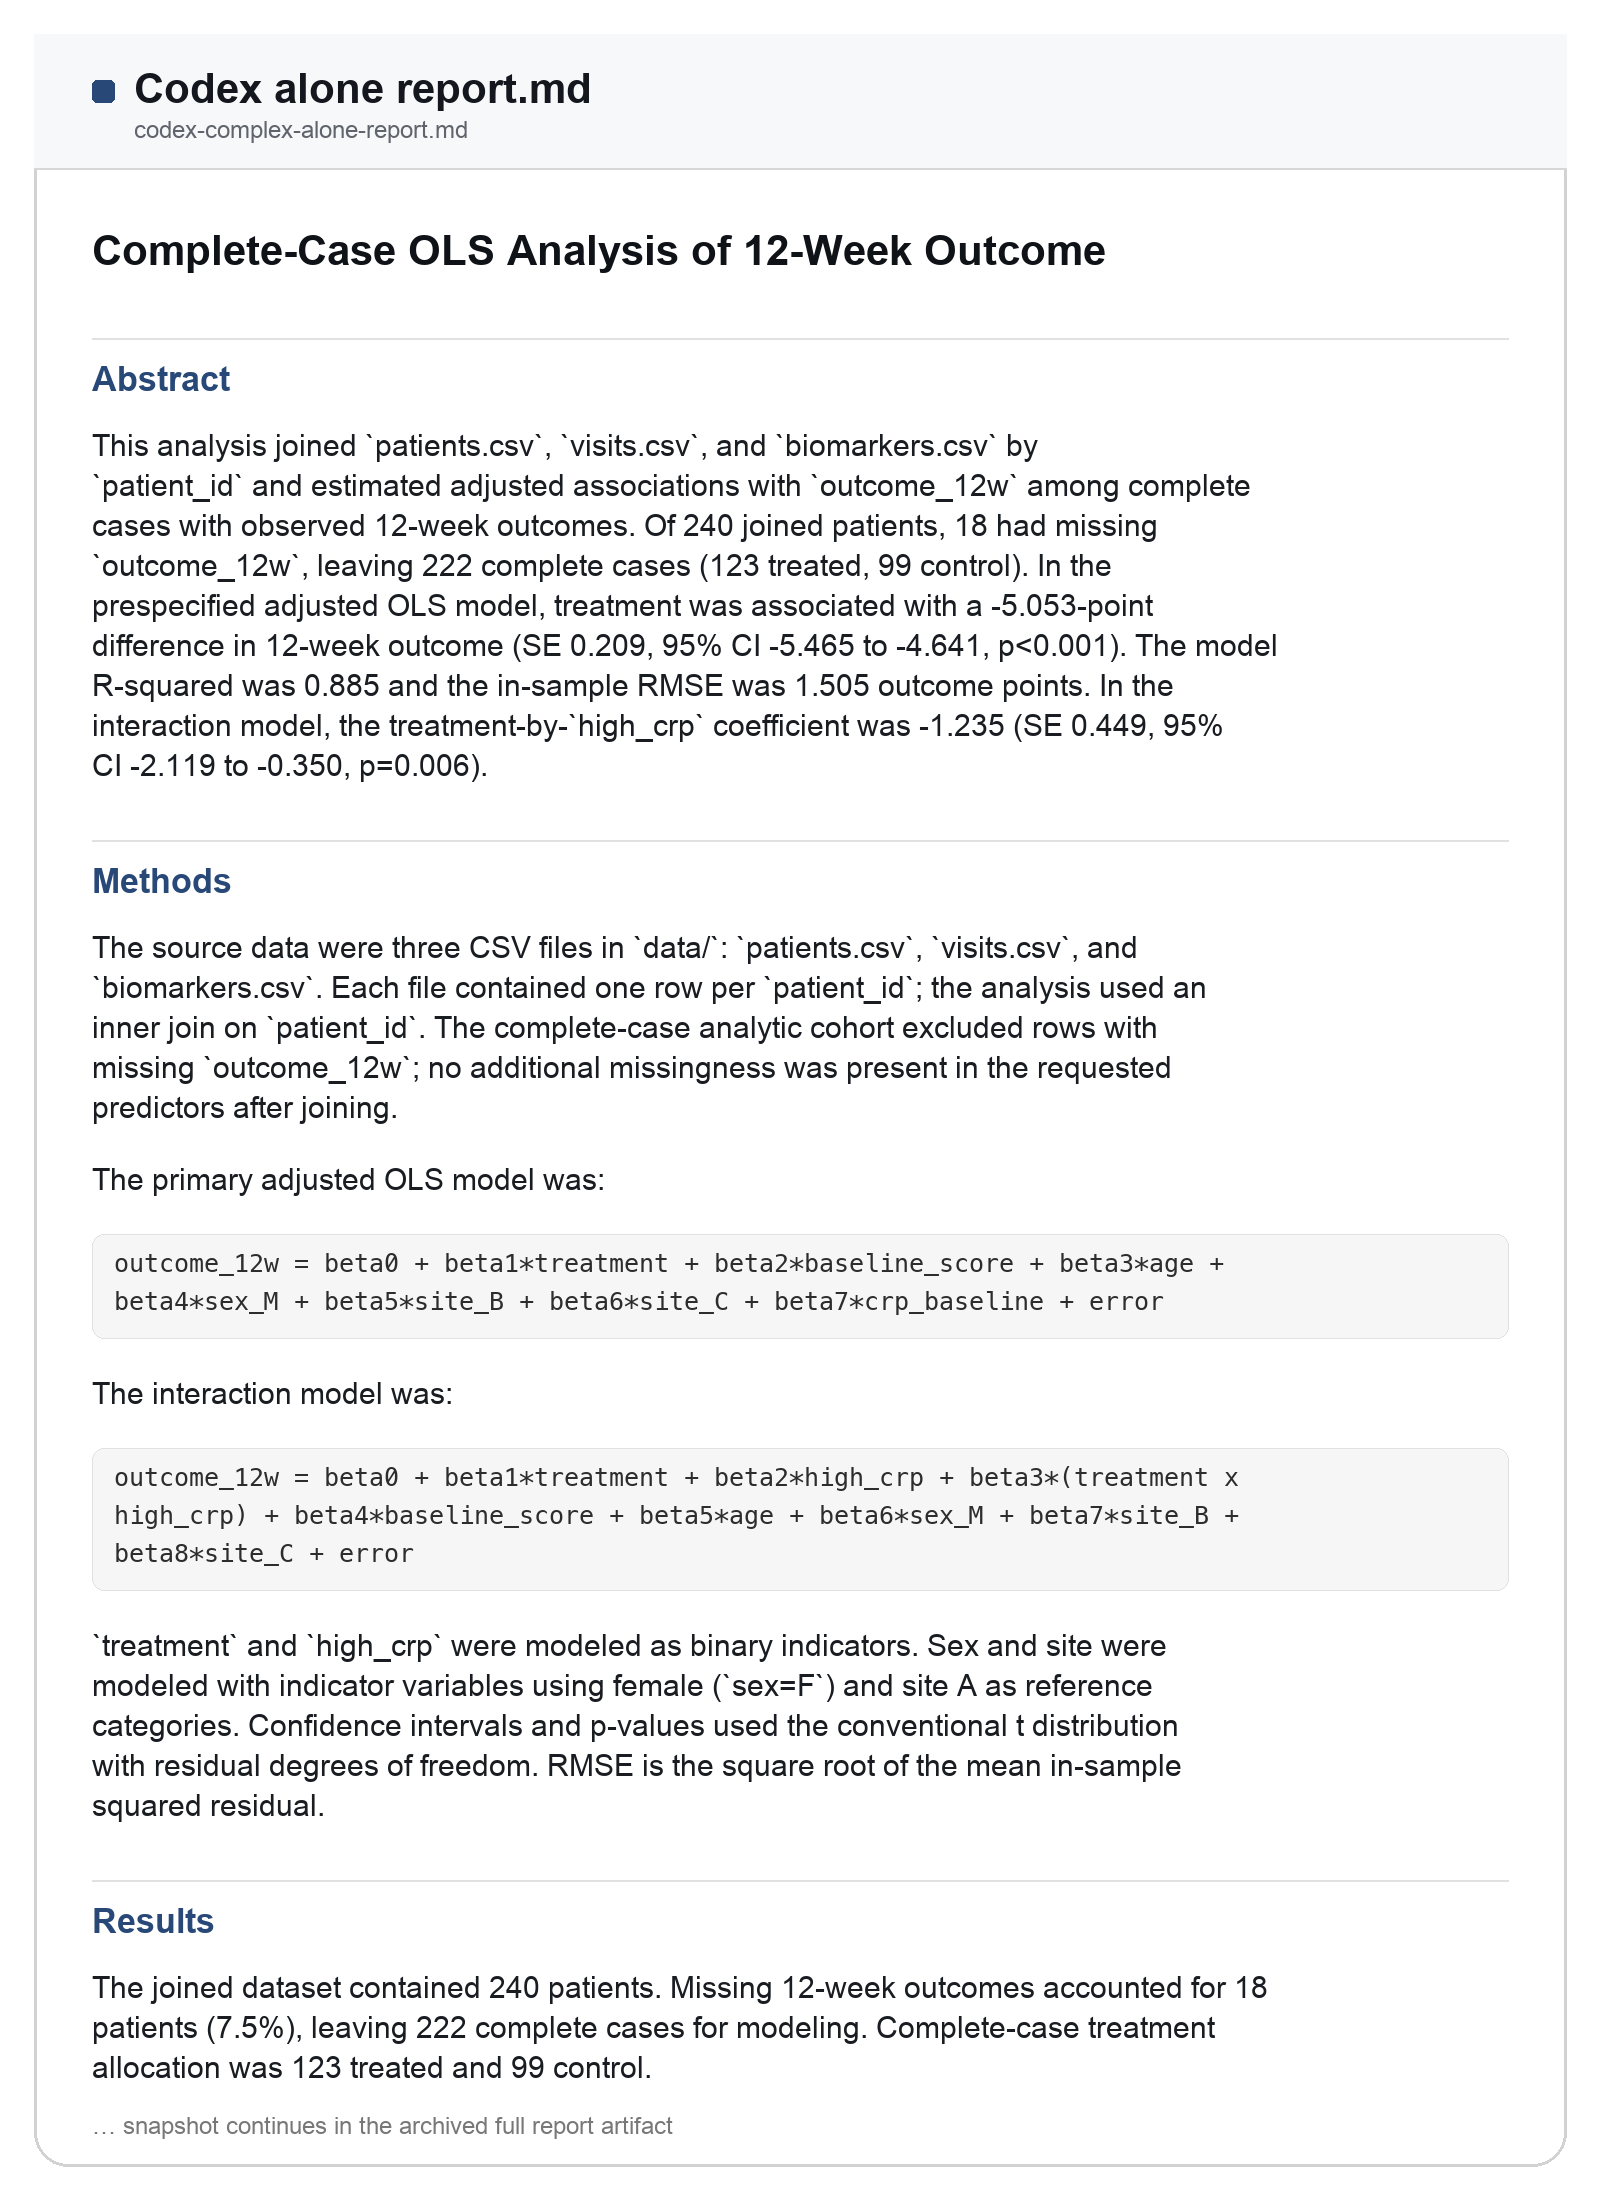
\includegraphics[width=0.48\textwidth]{figures/codex-alone-report-snapshot.png}\hfill
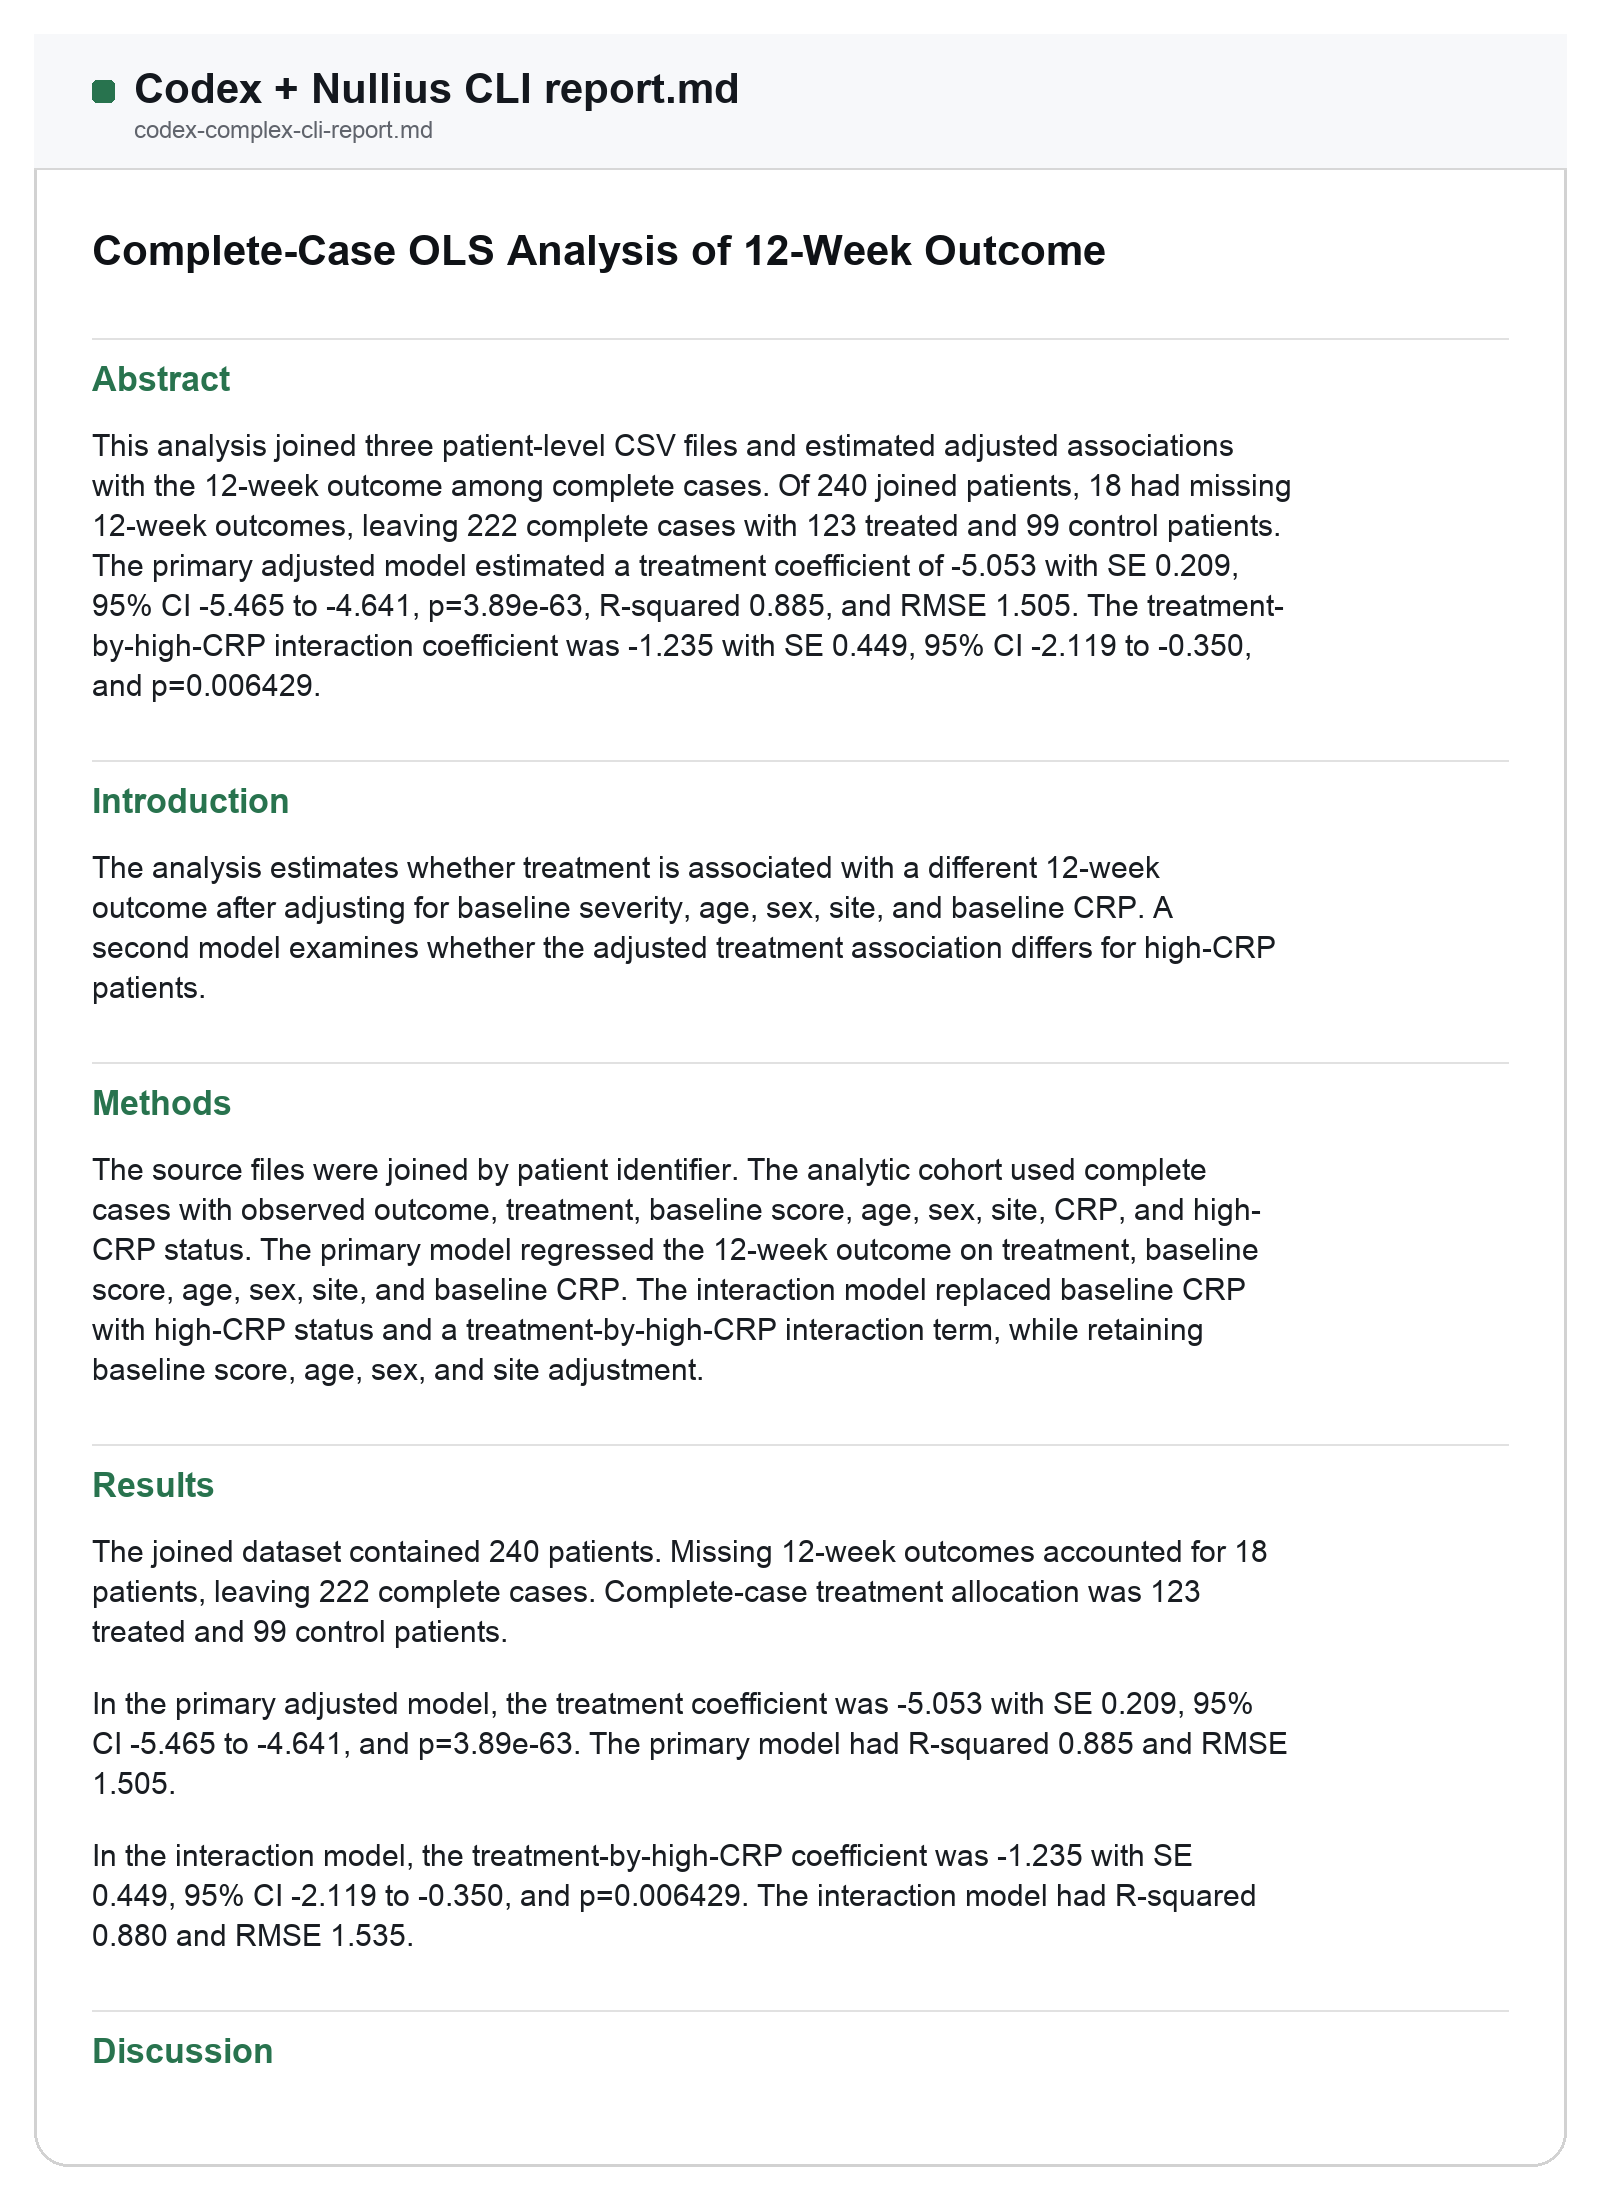
\includegraphics[width=0.48\textwidth]{figures/codex-nullius-report-snapshot.png}
\caption{Rendered snapshots of the two generated reports for the harder comparison. Left: the direct Codex report. Right: the report generated from the Nullius project state. The reports are not identical documents, but their substantive estimates agree to the displayed precision; the important difference is that only the right-hand report is backed by a project ledger that \texttt{verify} can certify.}
\label{fig:codex-report-snapshots}
\end{figure}

The harder reports show the same pattern under more realistic pressure. The Codex-alone report is again richer as a conventional free-standing manuscript: it spells out the model equations, reference categories, confidence-interval construction, residual degrees of freedom, and several limitations. The Nullius-backed report is shorter and closer to the evidence table: it reports the same cohort counts, coefficients, confidence intervals, $R^2$, and RMSE to the displayed precision, but it uses the exact p-values from the registered artifact and ends with explicit data/code artifact locations. Thus the observed tradeoff is not ``better writing versus worse writing.'' It is that an unconstrained coding agent can write a more discursive report, while Nullius makes the report stricter, less embellished, and easier to audit.

This stronger Codex run is exactly why the distinction matters. Codex did the analysis well and saved useful files, but when the report alone was imported into a blank Nullius project, \texttt{verify} still returned \texttt{ok: false}: readiness $0.4857$, supported claims 0, 15 ungrounded floating-point quantities, and seven ungrounded integers. In this paper, \emph{readiness} is Nullius' deterministic pre-export score: a manuscript is ready only when required sections are present, result claims are supported by accepted evidence, referenced artifacts exist, citations and markers are resolved, and no blocking gate failures remain. Thus a low readiness score does not mean Codex computed the wrong coefficients; it means the saved manuscript is not yet a machine-checkable research object.

In the gated condition, the same analysis script was run inside a Nullius project with warnings promoted to errors, the numeric artifacts were registered as execution evidence, two result claims were linked to that evidence, and the manuscript was written against a gate-readable metric artifact. \texttt{verify --json} returned \texttt{ok: true}, readiness $1.0$, two supported claims, zero ungrounded numbers, and no missing artifacts. For repository-disclosure reasons, this gated condition was driven by the current Codex session using the local Nullius CLI rather than by a second external Codex subprocess granted access to the repository; the recorded commands and artifacts are saved under \texttt{docs/paper/evaluation/}.

\begin{table}[h]
\centering
\small
\begin{tabular}{@{}p{0.25\textwidth}p{0.33\textwidth}p{0.33\textwidth}@{}}
\toprule
 & \textbf{Codex alone} & \textbf{Codex + Nullius CLI} \\
\midrule
Codex settings & \texttt{codex-cli 0.141.0}; model \texttt{gpt-5.5}; effort \texttt{xhigh} & current Codex session driving local Nullius CLI; same analysis script and gate inputs \\
Task complexity & three-table join, missing outcomes, complete-case filtering, adjusted OLS, interaction model & same task, but outputs had to become evidence, claims, and a gate-passing manuscript \\
Result values & treatment $-5.053$ (SE $0.209$), 95\% CI $[-5.465,-4.641]$, $R^2=0.885$; interaction $-1.235$ ($p=0.006$) & same displayed values, sourced from a gate-readable metric artifact \\
Runtime quality check & script ultimately passed \texttt{python3 -W error} after Codex fixed warning and prose issues & execution evidence records warning-as-error execution, exit code 0, artifact hashes, stdout, and stderr \\
Nullius audit & \texttt{verify} failed: readiness $0.4857$, supported claims 0 & \texttt{verify} passed: readiness $1.0$, supported claims 2 \\
Numeric grounding & 15 floating-point values and 7 integers ungrounded & 0 ungrounded result numbers, 0 ungrounded integers \\
\bottomrule
\end{tabular}
\caption{Harder harness comparison. Codex alone produced a high-quality analysis and even repaired its own script warnings, but the direct report was still not a gate-checkable research object. Nullius changed the persistence format of the same work, not the intelligence of the operator.}
\label{tab:codexcli2}
\end{table}

Four observations generalize. First, the routes failed \emph{differently}: the raw API call hallucinated the arithmetic itself, the ungated Codex harness computed both analyses correctly but left no durable evidence graph behind the prose, and the gated route made the correctness claim a property of the project state. Second, every recovery step in the gated route was driven by an external signal (an exit code, a reviewer finding, a gate rejection), consistent with the evidence that self-correction without such signals does not converge \cite{huang2024}. Third, a strong coding harness can and should remain in the loop: Codex or Claude Code is useful precisely because it can inspect files, repair scripts, and drive commands. Fourth, Nullius' role is narrower and more invariant: it supplies the layer that decides which claims may enter the manuscript.

\section{Limitations and Future Work}

Nullius enforces \emph{traceability}, not \emph{truth}. A grounded number can still be the output of a flawed analysis; a verified citation can still be interpreted tendentiously; deterministic gates cannot judge novelty or theoretical soundness, which remain with the reviewer role and the human. The claim--citation relevance check is advisory precisely because it is an LLM judgment. Reproducibility currently means ``re-runs on this machine now''; environment pinning (interpreter versions, package lockfiles, seeds) is future work, Section~\ref{sec:casestudy} is a first controlled comparison of gated and ungated generation; a systematic benchmark across many questions, datasets, and models remains the natural next step. Finally, the current scheduler parallelizes lanes but does not yet explore branches of a single lane in the style of tree-search agents \cite{aisci2}; the node versioning model was designed with that extension in mind.

\section{Conclusion}

The failures of autonomous research systems are not mysterious: they happen where model output is trusted without external evidence. Nullius shows that a small set of deterministic mechanisms --- an evidence bank fed only by real execution, a claim ledger typed against it, registry-backed citation checks, re-execution-based reproducibility, and gates that run at the moment of writing --- can be composed into a harness in which the convenient failure modes are simply unavailable, while independent review roles, sandboxed execution, and full-transcript observability handle what determinism cannot. \emph{Nullius in verba}: the machine's word alone is never enough, and the architecture makes sure it never has to be.

\begin{thebibliography}{9}
\small

\bibitem{huang2024}
J.~Huang et al.
\newblock Large language models cannot self-correct reasoning yet.
\newblock In \emph{Proc.\ ICLR}, 2024.

\bibitem{judge-bias}
L.~Zheng et al.
\newblock Judging LLM-as-a-judge with MT-Bench and Chatbot Arena.
\newblock In \emph{Proc.\ NeurIPS}, 2023.

\bibitem{self-pref}
A.~Panickssery, S.~Bowman, and S.~Feng.
\newblock LLM evaluators recognize and favor their own generations.
\newblock In \emph{Proc.\ NeurIPS}, 2024.

\bibitem{aisci2}
Y.~Yamada et al.
\newblock The AI Scientist-v2: workshop-level automated scientific discovery via agentic tree search.
\newblock \emph{arXiv:2504.08066}, 2025.

\bibitem{beel2025}
J.~Beel, M.-Y.~Kan, and M.~Baumgart.
\newblock Evaluating Sakana's AI Scientist for autonomous research: wishful thinking or an emerging reality towards `Artificial Research Intelligence' (ARI)?
\newblock \emph{arXiv:2502.14297}, 2025.

\bibitem{sandbox-eval}
R.~Rabin, J.~Hostetler, S.~McGregor, B.~Weir, and N.~Judd.
\newblock SandboxEval: towards securing test environment for untrusted code.
\newblock \emph{arXiv:2504.00018}, 2025.

\bibitem{anthropic-agents}
Anthropic.
\newblock How we built our multi-agent research system.
\newblock Engineering blog, \url{https://www.anthropic.com/engineering/multi-agent-research-system}, 2025.

\end{thebibliography}

\end{document}
